
\documentclass{article} % For LaTeX2e
%\usepackage{format/nips13submit_e}
%\nipsfinalcopy % Uncomment for camera-ready version
\usepackage{times}
\usepackage{hyperref}
\usepackage{url}
\usepackage{color}
\definecolor{mydarkblue}{rgb}{0,0.08,0.45}
\hypersetup{
    pdfpagemode=UseNone,
    colorlinks=true,
    linkcolor=mydarkblue,
    citecolor=mydarkblue,
    filecolor=mydarkblue,
    urlcolor=mydarkblue,
    pdfview=FitH}

\usepackage{graphicx, amsmath, amsfonts, bm, lipsum, capt-of}

\usepackage{natbib, xcolor, wrapfig, booktabs, multirow, caption}

\usepackage{float}

\def\ie{i.e.\ }
\def\eg{e.g.\ }

\title{An automatic report for the dataset : stocks-0-hyundaimobis}

\author{
The Automatic Statistician
}

\newcommand{\fix}{\marginpar{FIX}}
\newcommand{\new}{\marginpar{NEW}}

\setlength{\marginparwidth}{0.9in}
%\input{include/commenting.tex}

%% For submission, make all render blank.
%\renewcommand{\LATER}[1]{}
%\renewcommand{\fLATER}[1]{}
%\renewcommand{\TBD}[1]{}
%\renewcommand{\fTBD}[1]{}
%\renewcommand{\PROBLEM}[1]{}
%\renewcommand{\fPROBLEM}[1]{}
%\renewcommand{\NA}[1]{#1}  % Note, NA's pass through!

\begin{document}

\allowdisplaybreaks

\maketitle

\begin{abstract}
This report was produced by the Automatic Bayesian Covariance Discovery (ABCD) algorithm.
%See \url{http://arxiv.org/abs/1302.4922} and \url{http://www-kd.iai.uni-bonn.de/cml/proceedings/papers/2.pdf} for preliminary papers.
\end{abstract}

\section{Executive summary}

The raw data and full model posterior with extrapolations are shown in figure~\ref{fig:rawandfit}.

\begin{figure}[H]
\newcommand{\wmgd}{0.5\columnwidth}
\newcommand{\hmgd}{3.0cm}
\newcommand{\mdrd}{stocks-0-hyundaimobis}
\newcommand{\mbm}{\hspace{-0.3cm}}
\begin{tabular}{cc}
\mbm 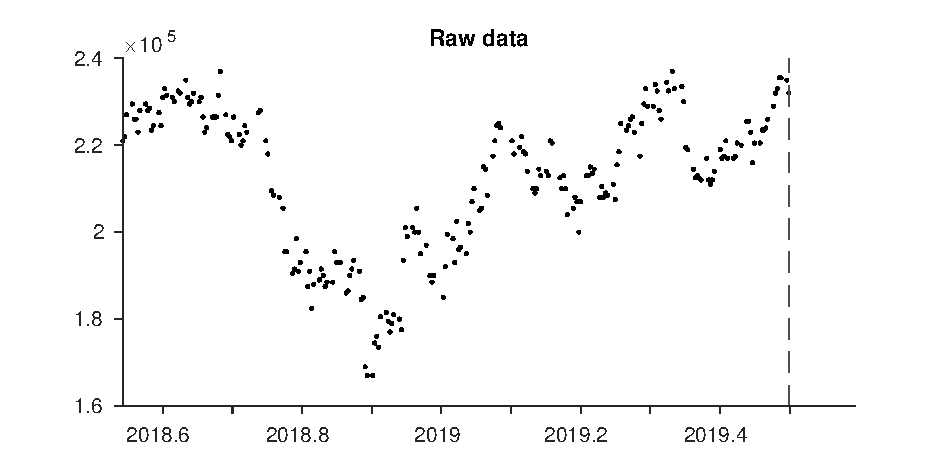
\includegraphics[width=\wmgd,height=\hmgd]{\mdrd/stocks-0-hyundaimobis_raw_data} & 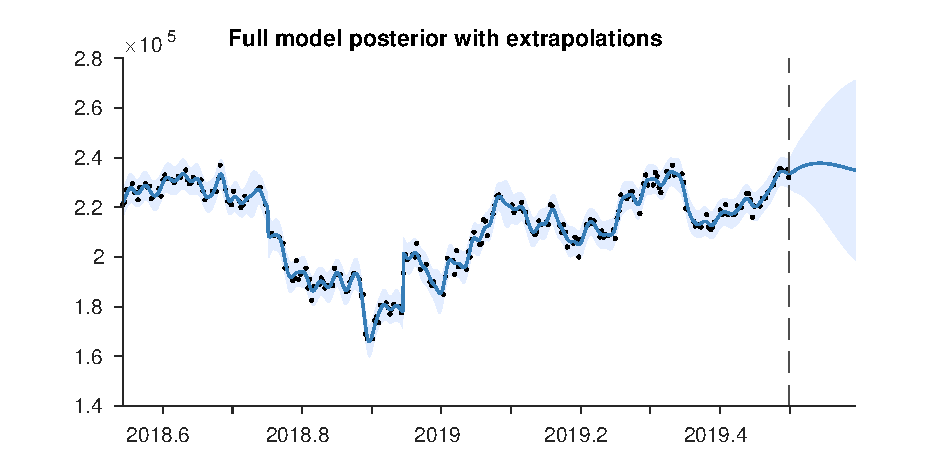
\includegraphics[width=\wmgd,height=\hmgd]{\mdrd/stocks-0-hyundaimobis_all}
\end{tabular}
\caption{Raw data (left) and model posterior with extrapolation (right)}
\label{fig:rawandfit}
\end{figure}

The structure search algorithm has identified six additive components in the data.
The  first 3 additive components explain 93.2\% of the variation in the data as shown by the coefficient of determination ($R^2$) values in table~\ref{table:stats}.
The  first 5 additive components explain 100.0\% of the variation in the data.
After the first 4 components the cross validated mean absolute error (MAE) does not decrease by more than 0.1\%.
This suggests that subsequent terms are modelling very short term trends, uncorrelated noise or are artefacts of the model or search procedure.
Short summaries of the additive components are as follows:
\begin{itemize}

  \item A very smooth function. This function applies until 21 Nov 2018 and from 21 Nov 2018 onwards. 

  \item A smooth function. This function applies from 20 Sep 2018 until 21 Nov 2018 and from 21 Nov 2018 until 29 Nov 2018. 

  \item A smooth function. This function applies until 20 Sep 2018 and from 29 Nov 2018 onwards. 

  \item A smooth function. This function applies from 21 Nov 2018 until 21 Nov 2018. 

  \item Uncorrelated noise. 

  \item A constant. 

\end{itemize}

\begin{table}[htb]
\begin{center}
{\small
\begin{tabular}{|r|rrrrr|}
\hline
\bf{\#} & {$R^2$ (\%)} & {$\Delta R^2$ (\%)} & {Residual $R^2$ (\%)} & {Cross validated MAE} & Reduction in MAE (\%)\\
\hline
- & - & - & - & 212010.68 & -\\

1 & 50.8 & 50.8 & 50.8 & 9676.31 & 95.4\\

2 & 77.2 & 26.4 & 53.6 & 6993.08 & 27.7\\

3 & 93.2 & 16.0 & 70.0 & 5548.71 & 20.7\\

4 & 98.7 & 5.5 & 80.8 & 5416.36 & 2.4\\

5 & 100.0 & 1.3 & 100.0 & 5416.36 & 0.0\\

6 & 100.0 & 0.0 & 4.4 & 5416.48 & -0.0\\

\hline
\end{tabular}
\caption{
Summary statistics for cumulative additive fits to the data.
The residual coefficient of determination ($R^2$) values are computed using the residuals from the previous fit as the target values; this measures how much of the residual variance is explained by each new component.
The mean absolute error (MAE) is calculated using 10 fold cross validation with a contiguous block design; this measures the ability of the model to interpolate and extrapolate over moderate distances.
The model is fit using the full data and the MAE values are calculated using this model; this double use of data means that the MAE values cannot be used reliably as an estimate of out-of-sample predictive performance.
}
\label{table:stats}
}
\end{center}
\end{table}

Model checking statistics are summarised in table~\ref{table:check} in section~\ref{sec:check}.
These statistics have not revealed any inconsistencies between the model and observed data.

The rest of the document is structured as follows.
In section~\ref{sec:discussion} the forms of the additive components are described and their posterior distributions are displayed.
In section~\ref{sec:extrap} the modelling assumptions of each component are discussed with reference to how this affects the extrapolations made by the model.
Section~\ref{sec:check} discusses model checking statistics, with plots showing the form of any detected discrepancies between the model and observed data.

\section{Detailed discussion of additive components}
\label{sec:discussion}

\subsection{Component 1 : A very smooth function. This function applies until 21 Nov 2018 and from 21 Nov 2018 onwards}

This component is a very smooth function.
This component applies until 21 Nov 2018 and from 21 Nov 2018 onwards.

This component explains 50.8\% of the total variance.
The addition of this component reduces the cross validated MAE by 95.4\% from 212010.7 to 9676.3.


\begin{figure}[H]
\newcommand{\wmgd}{0.5\columnwidth}
\newcommand{\hmgd}{3.0cm}
\newcommand{\mdrd}{stocks-0-hyundaimobis}
\newcommand{\mbm}{\hspace{-0.3cm}}
\begin{tabular}{cc}
\mbm 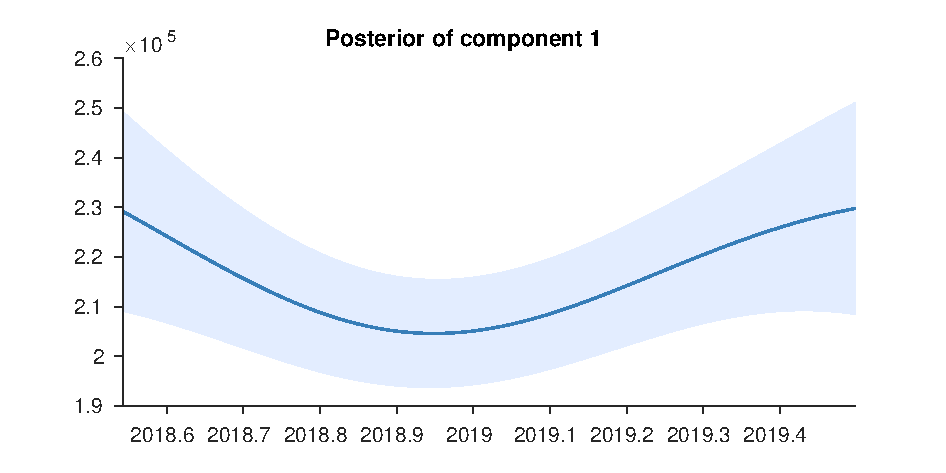
\includegraphics[width=\wmgd,height=\hmgd]{\mdrd/stocks-0-hyundaimobis_1} & 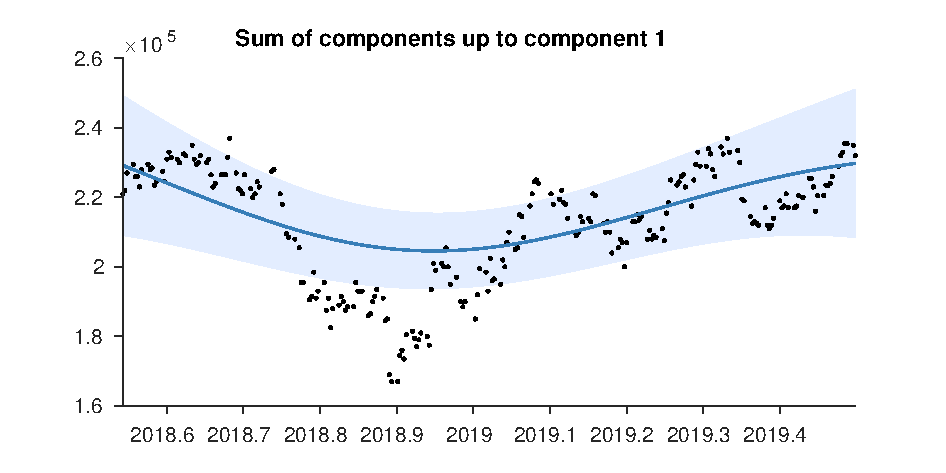
\includegraphics[width=\wmgd,height=\hmgd]{\mdrd/stocks-0-hyundaimobis_1_cum}
\end{tabular}
\caption{Pointwise posterior of component 1 (left) and the posterior of the cumulative sum of components with data (right)}
\label{fig:comp1}
\end{figure}

\begin{figure}[H]
\newcommand{\wmgd}{0.5\columnwidth}
\newcommand{\hmgd}{3.0cm}
\newcommand{\mdrd}{stocks-0-hyundaimobis}
\newcommand{\mbm}{\hspace{-0.3cm}}
\begin{tabular}{cc}
\mbm 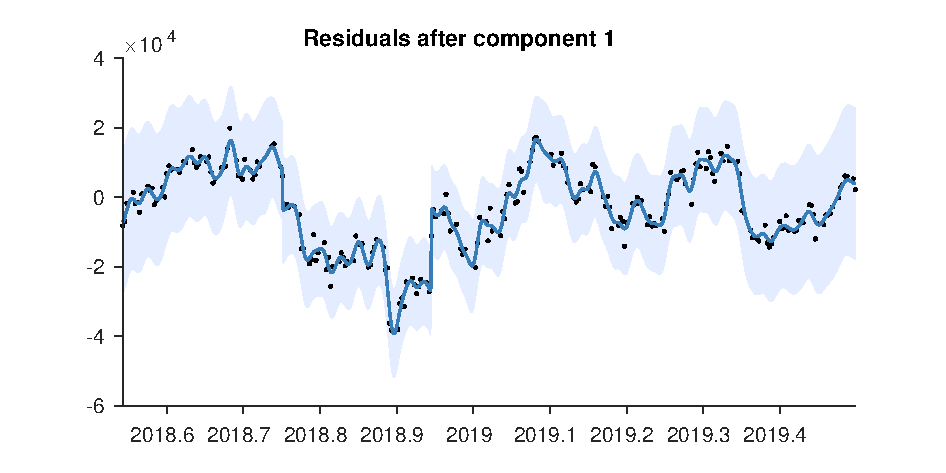
\includegraphics[width=\wmgd,height=\hmgd]{\mdrd/stocks-0-hyundaimobis_1_anti_cum}
\end{tabular}
\caption{Pointwise posterior of residuals after adding component 1}
\label{fig:comp1}
\end{figure}

\subsection{Component 2 : A smooth function. This function applies from 20 Sep 2018 until 21 Nov 2018 and from 21 Nov 2018 until 29 Nov 2018}

This component is a smooth function with a typical lengthscale of 4.9 weeks.
This component applies from 20 Sep 2018 until 21 Nov 2018 and from 21 Nov 2018 until 29 Nov 2018.

This component explains 53.6\% of the residual variance; this increases the total variance explained from 50.8\% to 77.2\%.
The addition of this component reduces the cross validated MAE by 27.73\% from 9676.31 to 6993.08.


\begin{figure}[H]
\newcommand{\wmgd}{0.5\columnwidth}
\newcommand{\hmgd}{3.0cm}
\newcommand{\mdrd}{stocks-0-hyundaimobis}
\newcommand{\mbm}{\hspace{-0.3cm}}
\begin{tabular}{cc}
\mbm 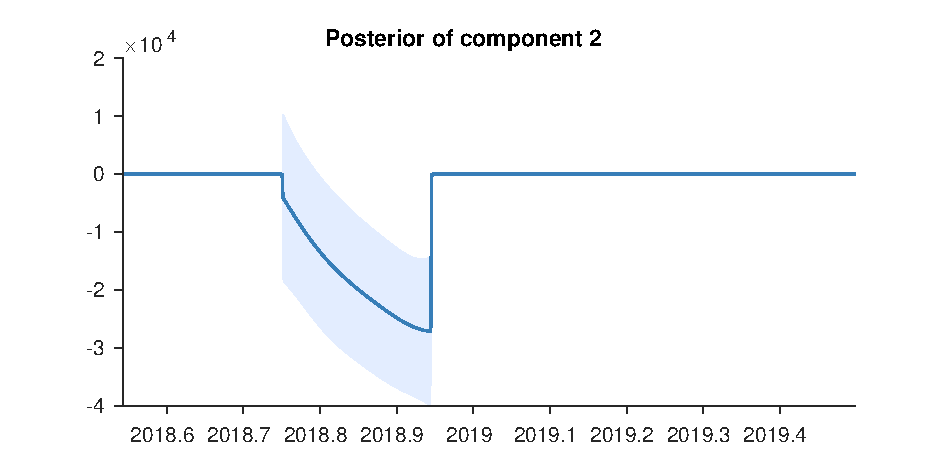
\includegraphics[width=\wmgd,height=\hmgd]{\mdrd/stocks-0-hyundaimobis_2} & 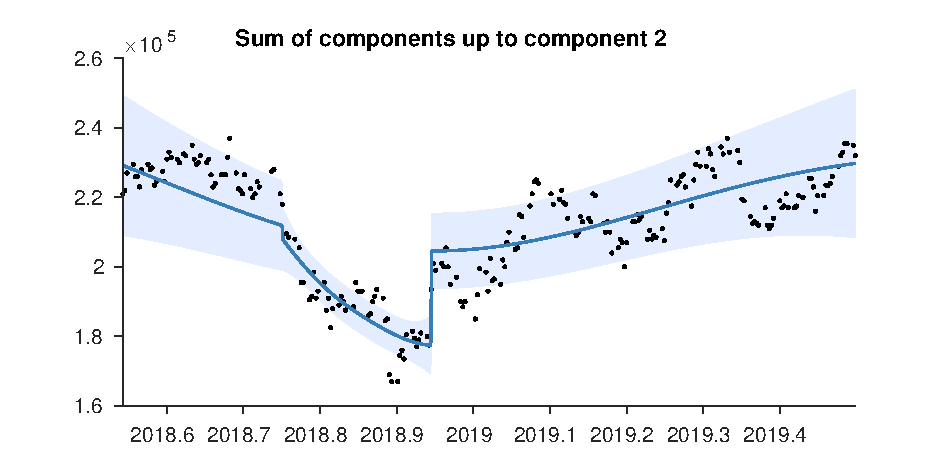
\includegraphics[width=\wmgd,height=\hmgd]{\mdrd/stocks-0-hyundaimobis_2_cum}
\end{tabular}
\caption{Pointwise posterior of component 2 (left) and the posterior of the cumulative sum of components with data (right)}
\label{fig:comp2}
\end{figure}

\begin{figure}[H]
\newcommand{\wmgd}{0.5\columnwidth}
\newcommand{\hmgd}{3.0cm}
\newcommand{\mdrd}{stocks-0-hyundaimobis}
\newcommand{\mbm}{\hspace{-0.3cm}}
\begin{tabular}{cc}
\mbm 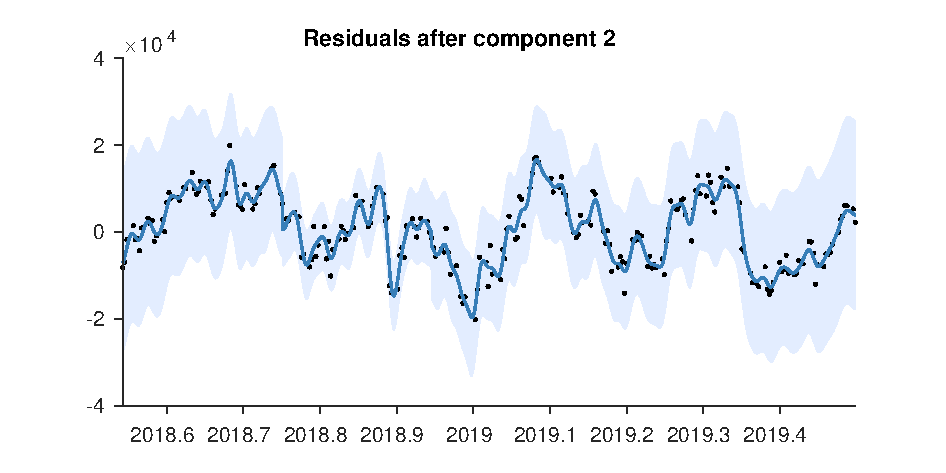
\includegraphics[width=\wmgd,height=\hmgd]{\mdrd/stocks-0-hyundaimobis_2_anti_cum}
\end{tabular}
\caption{Pointwise posterior of residuals after adding component 2}
\label{fig:comp2}
\end{figure}

\subsection{Component 3 : A smooth function. This function applies until 20 Sep 2018 and from 29 Nov 2018 onwards}

This component is a smooth function with a typical lengthscale of 3.1 weeks.
This component applies until 20 Sep 2018 and from 29 Nov 2018 onwards.

This component explains 70.0\% of the residual variance; this increases the total variance explained from 77.2\% to 93.2\%.
The addition of this component reduces the cross validated MAE by 20.65\% from 6993.08 to 5548.71.


\begin{figure}[H]
\newcommand{\wmgd}{0.5\columnwidth}
\newcommand{\hmgd}{3.0cm}
\newcommand{\mdrd}{stocks-0-hyundaimobis}
\newcommand{\mbm}{\hspace{-0.3cm}}
\begin{tabular}{cc}
\mbm 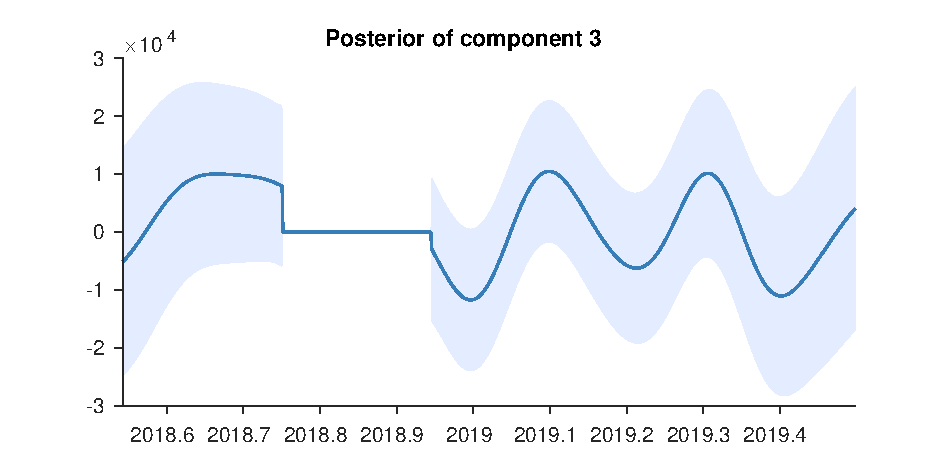
\includegraphics[width=\wmgd,height=\hmgd]{\mdrd/stocks-0-hyundaimobis_3} & 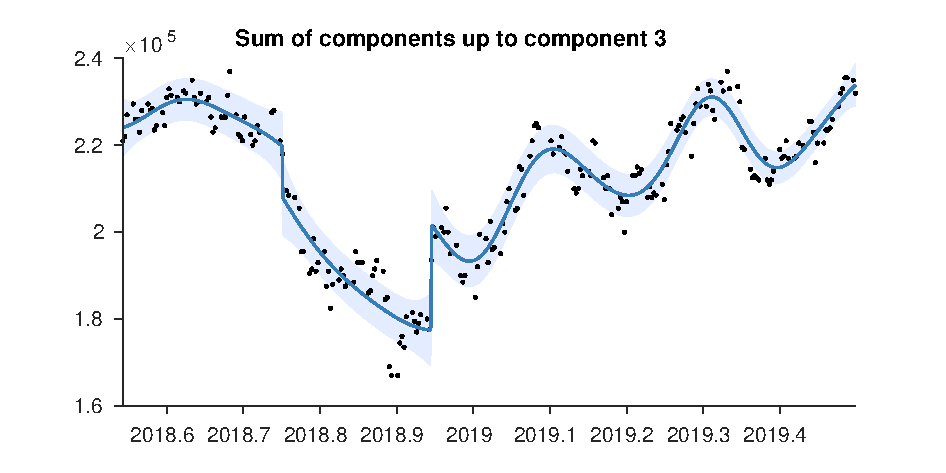
\includegraphics[width=\wmgd,height=\hmgd]{\mdrd/stocks-0-hyundaimobis_3_cum}
\end{tabular}
\caption{Pointwise posterior of component 3 (left) and the posterior of the cumulative sum of components with data (right)}
\label{fig:comp3}
\end{figure}

\begin{figure}[H]
\newcommand{\wmgd}{0.5\columnwidth}
\newcommand{\hmgd}{3.0cm}
\newcommand{\mdrd}{stocks-0-hyundaimobis}
\newcommand{\mbm}{\hspace{-0.3cm}}
\begin{tabular}{cc}
\mbm 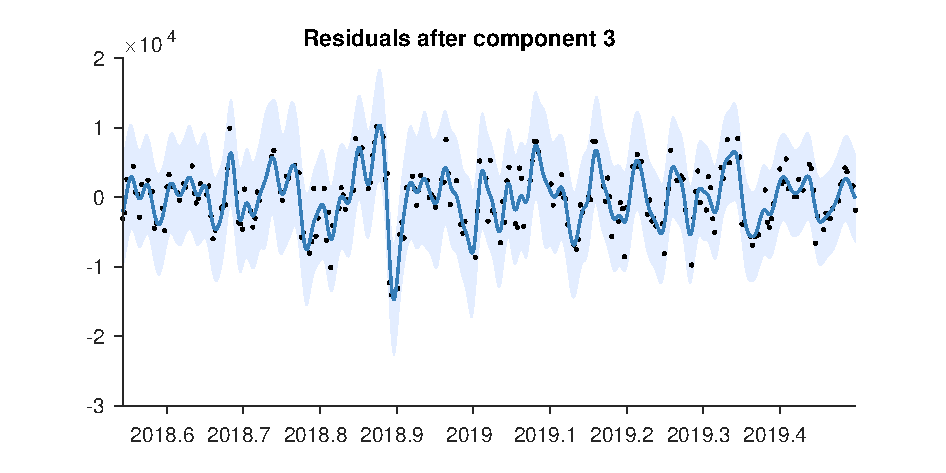
\includegraphics[width=\wmgd,height=\hmgd]{\mdrd/stocks-0-hyundaimobis_3_anti_cum}
\end{tabular}
\caption{Pointwise posterior of residuals after adding component 3}
\label{fig:comp3}
\end{figure}

\subsection{Component 4 : A smooth function. This function applies from 21 Nov 2018 until 21 Nov 2018}

This component is a smooth function with a typical lengthscale of 2.6 days.
This component applies from 21 Nov 2018 until 21 Nov 2018.

This component explains 80.8\% of the residual variance; this increases the total variance explained from 93.2\% to 98.7\%.
The addition of this component reduces the cross validated MAE by 2.39\% from 5548.71 to 5416.36.


\begin{figure}[H]
\newcommand{\wmgd}{0.5\columnwidth}
\newcommand{\hmgd}{3.0cm}
\newcommand{\mdrd}{stocks-0-hyundaimobis}
\newcommand{\mbm}{\hspace{-0.3cm}}
\begin{tabular}{cc}
\mbm 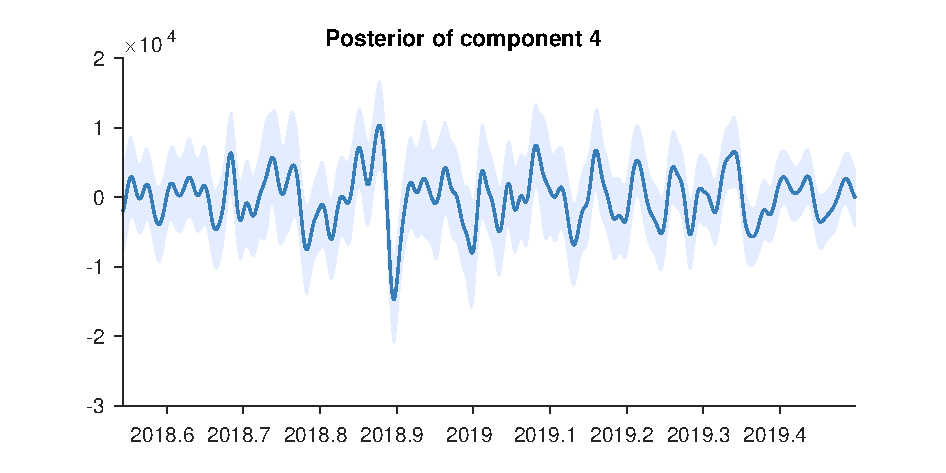
\includegraphics[width=\wmgd,height=\hmgd]{\mdrd/stocks-0-hyundaimobis_4} & 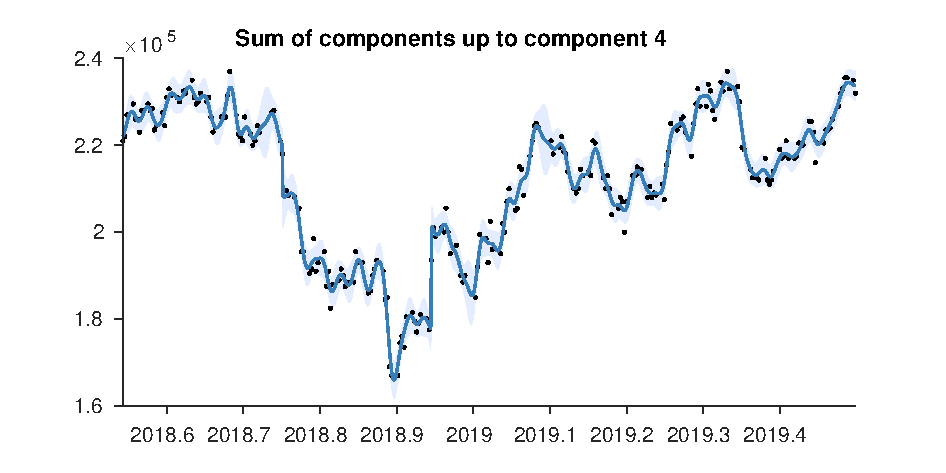
\includegraphics[width=\wmgd,height=\hmgd]{\mdrd/stocks-0-hyundaimobis_4_cum}
\end{tabular}
\caption{Pointwise posterior of component 4 (left) and the posterior of the cumulative sum of components with data (right)}
\label{fig:comp4}
\end{figure}

\begin{figure}[H]
\newcommand{\wmgd}{0.5\columnwidth}
\newcommand{\hmgd}{3.0cm}
\newcommand{\mdrd}{stocks-0-hyundaimobis}
\newcommand{\mbm}{\hspace{-0.3cm}}
\begin{tabular}{cc}
\mbm 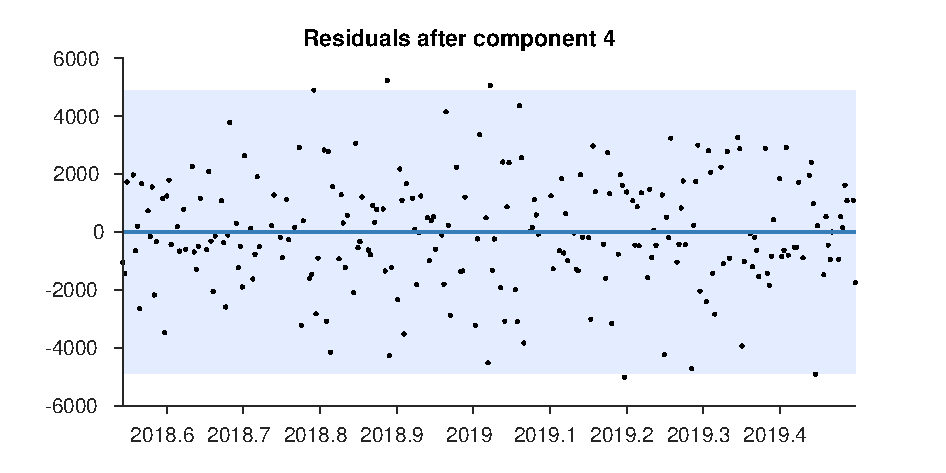
\includegraphics[width=\wmgd,height=\hmgd]{\mdrd/stocks-0-hyundaimobis_4_anti_cum}
\end{tabular}
\caption{Pointwise posterior of residuals after adding component 4}
\label{fig:comp4}
\end{figure}

\subsection{Component 5 : Uncorrelated noise}

This component models uncorrelated noise.

This component explains 100.0\% of the residual variance; this increases the total variance explained from 98.7\% to 100.0\%.
The addition of this component reduces the cross validated MAE by 0.00\% from 5416.36 to 5416.36.
This component explains residual variance but does not improve MAE which suggests that this component describes very short term patterns, uncorrelated noise or is an artefact of the model or search procedure.

\begin{figure}[H]
\newcommand{\wmgd}{0.5\columnwidth}
\newcommand{\hmgd}{3.0cm}
\newcommand{\mdrd}{stocks-0-hyundaimobis}
\newcommand{\mbm}{\hspace{-0.3cm}}
\begin{tabular}{cc}
\mbm 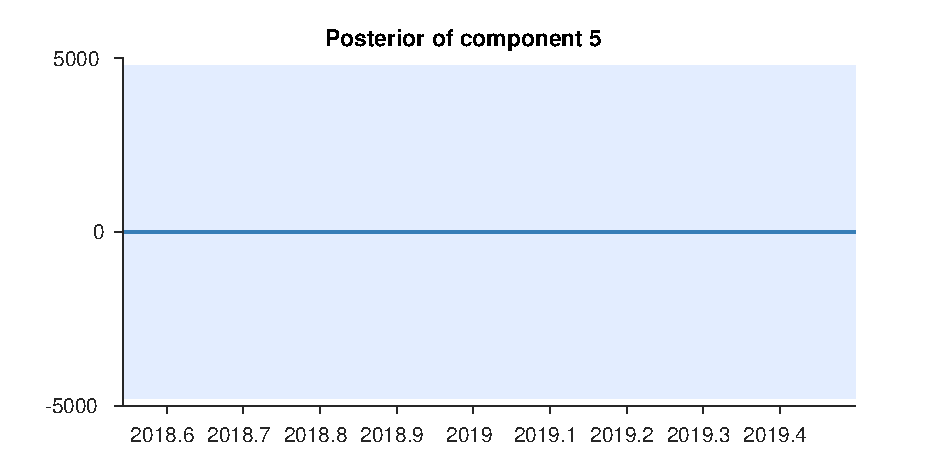
\includegraphics[width=\wmgd,height=\hmgd]{\mdrd/stocks-0-hyundaimobis_5} & 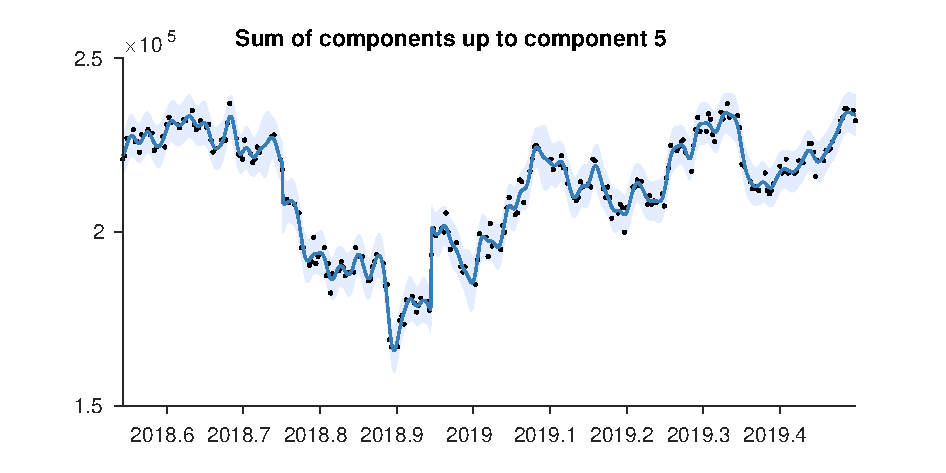
\includegraphics[width=\wmgd,height=\hmgd]{\mdrd/stocks-0-hyundaimobis_5_cum}
\end{tabular}
\caption{Pointwise posterior of component 5 (left) and the posterior of the cumulative sum of components with data (right)}
\label{fig:comp5}
\end{figure}

\begin{figure}[H]
\newcommand{\wmgd}{0.5\columnwidth}
\newcommand{\hmgd}{3.0cm}
\newcommand{\mdrd}{stocks-0-hyundaimobis}
\newcommand{\mbm}{\hspace{-0.3cm}}
\begin{tabular}{cc}
\mbm 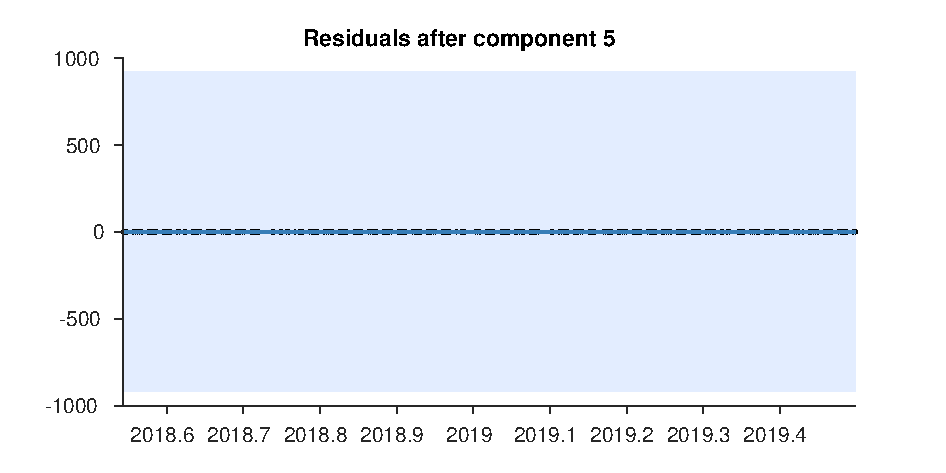
\includegraphics[width=\wmgd,height=\hmgd]{\mdrd/stocks-0-hyundaimobis_5_anti_cum}
\end{tabular}
\caption{Pointwise posterior of residuals after adding component 5}
\label{fig:comp5}
\end{figure}

\subsection{Component 6 : A constant}

This component is constant.

This component explains 4.4\% of the residual variance; this increases the total variance explained from 100.0\% to 100.0\%.
The addition of this component increases the cross validated MAE by 0.00\% from 5416.36 to 5416.48.
This component explains residual variance but does not improve MAE which suggests that this component describes very short term patterns, uncorrelated noise or is an artefact of the model or search procedure.

\begin{figure}[H]
\newcommand{\wmgd}{0.5\columnwidth}
\newcommand{\hmgd}{3.0cm}
\newcommand{\mdrd}{stocks-0-hyundaimobis}
\newcommand{\mbm}{\hspace{-0.3cm}}
\begin{tabular}{cc}
\mbm 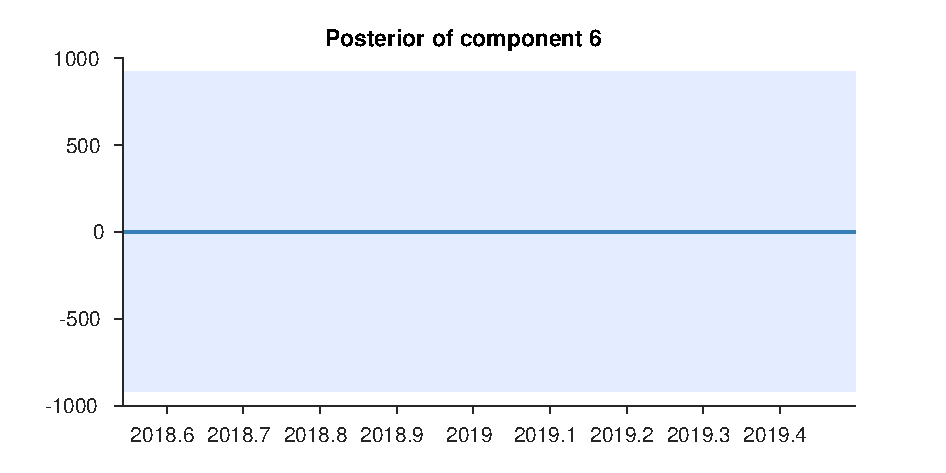
\includegraphics[width=\wmgd,height=\hmgd]{\mdrd/stocks-0-hyundaimobis_6} & 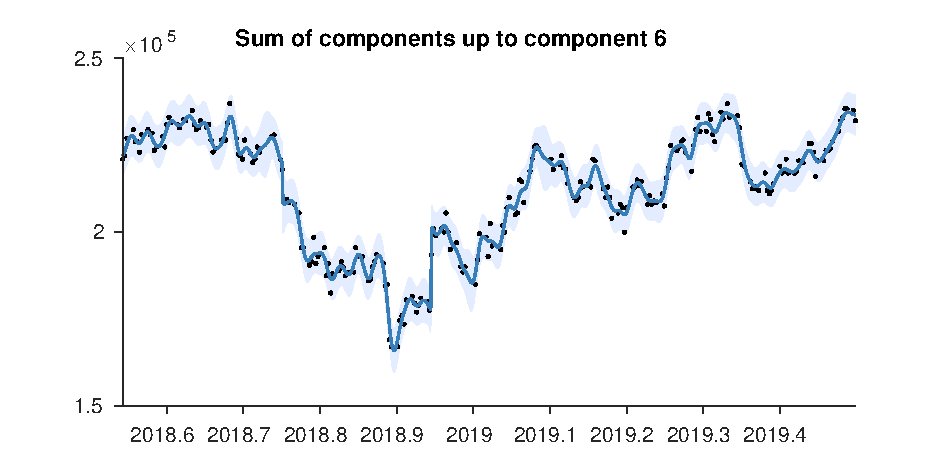
\includegraphics[width=\wmgd,height=\hmgd]{\mdrd/stocks-0-hyundaimobis_6_cum}
\end{tabular}
\caption{Pointwise posterior of component 6 (left) and the posterior of the cumulative sum of components with data (right)}
\label{fig:comp6}
\end{figure}

\section{Extrapolation}
\label{sec:extrap}

Summaries of the posterior distribution of the full model are shown in figure~\ref{fig:extrap}.
The plot on the left displays the mean of the posterior together with pointwise variance.
The plot on the right displays three random samples from the posterior.

\begin{figure}[H]
\newcommand{\wmgd}{0.5\columnwidth}
\newcommand{\hmgd}{3.0cm}
\newcommand{\mdrd}{stocks-0-hyundaimobis}
\newcommand{\mbm}{\hspace{-0.3cm}}
\begin{tabular}{cc}
\mbm 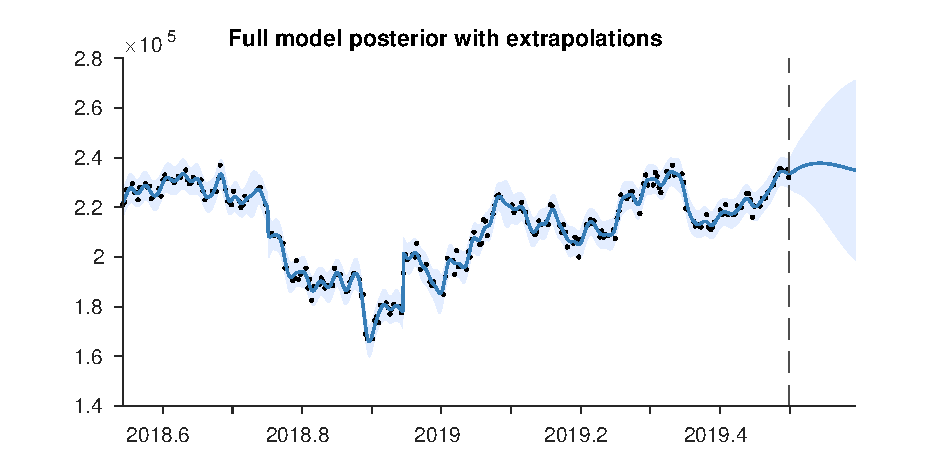
\includegraphics[width=\wmgd,height=\hmgd]{\mdrd/stocks-0-hyundaimobis_all} & 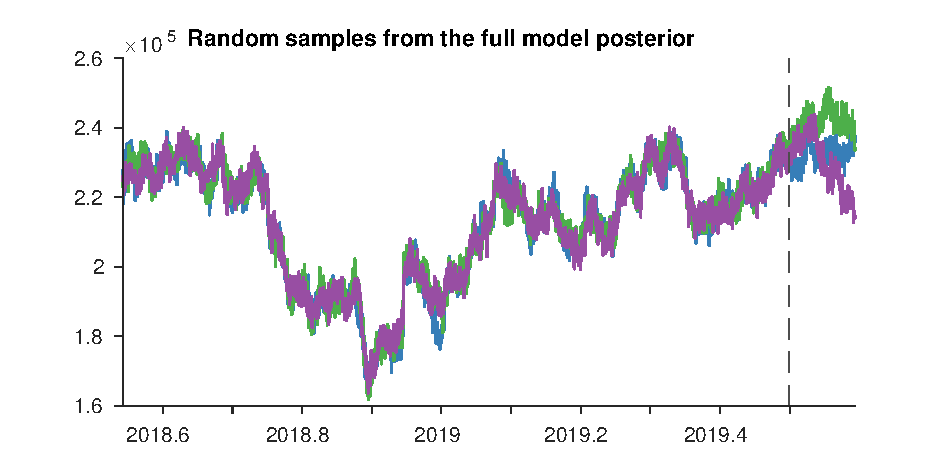
\includegraphics[width=\wmgd,height=\hmgd]{\mdrd/stocks-0-hyundaimobis_all_sample}
\end{tabular}
\caption{Full model posterior with extrapolation. Mean and pointwise variance (left) and three random samples (right)}
\label{fig:extrap}
\end{figure}

Below are descriptions of the modelling assumptions associated with each additive component and how they affect the predictive posterior.
Plots of the pointwise posterior and samples from the posterior are also presented, showing extrapolations from each component and the cuulative sum of components.

\subsection{Component 1 : A very smooth function. This function applies until 21 Nov 2018 and from 21 Nov 2018 onwards}

This component is assumed to continue very smoothly but is also assumed to be stationary so its distribution will eventually return to the prior.
The prior distribution places mass on smooth functions with a marginal mean of zero and a typical lengthscale of 2.0 years.
[This is a placeholder for a description of how quickly the posterior will start to resemble the prior].

\begin{figure}[H]
\newcommand{\wmgd}{0.5\columnwidth}
\newcommand{\hmgd}{3.0cm}
\newcommand{\mdrd}{stocks-0-hyundaimobis}
\newcommand{\mbm}{\hspace{-0.3cm}}
\begin{tabular}{cc}
\mbm 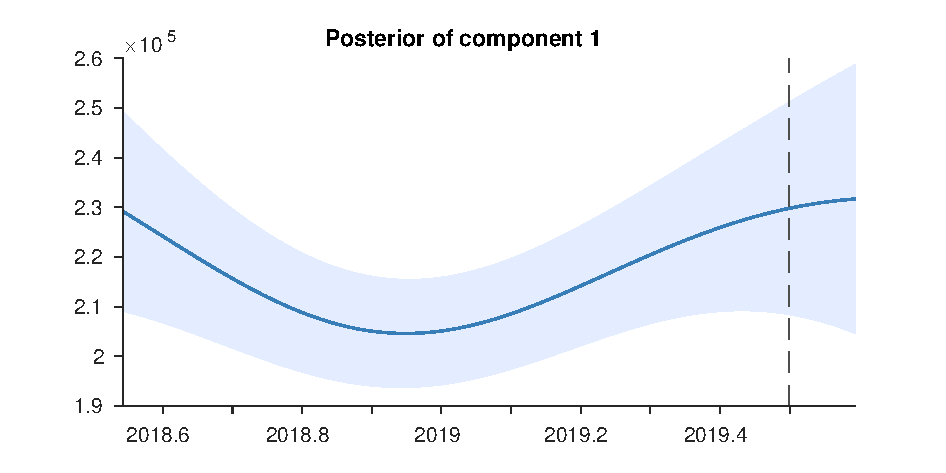
\includegraphics[width=\wmgd,height=\hmgd]{\mdrd/stocks-0-hyundaimobis_1_extrap} & 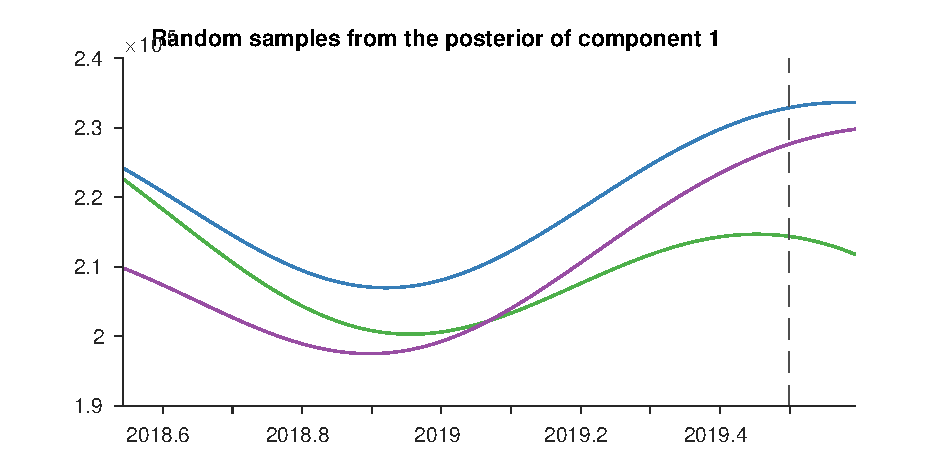
\includegraphics[width=\wmgd,height=\hmgd]{\mdrd/stocks-0-hyundaimobis_1_sample} \\
\mbm 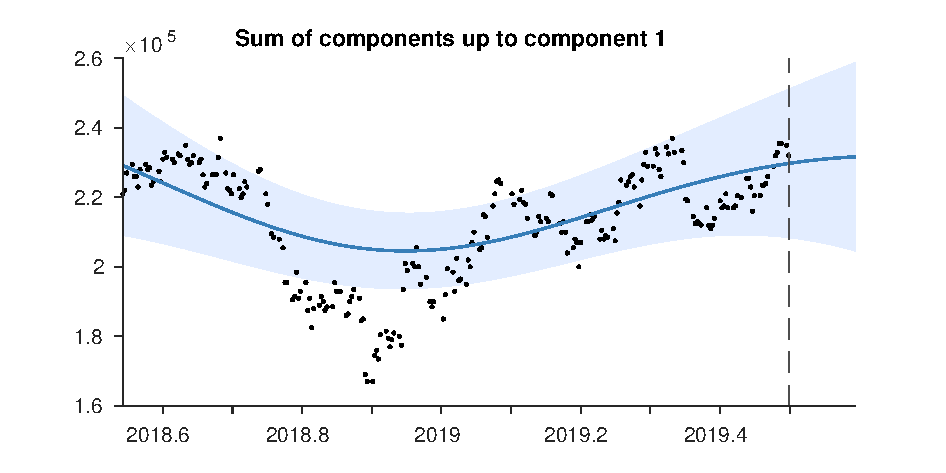
\includegraphics[width=\wmgd,height=\hmgd]{\mdrd/stocks-0-hyundaimobis_1_cum_extrap} & 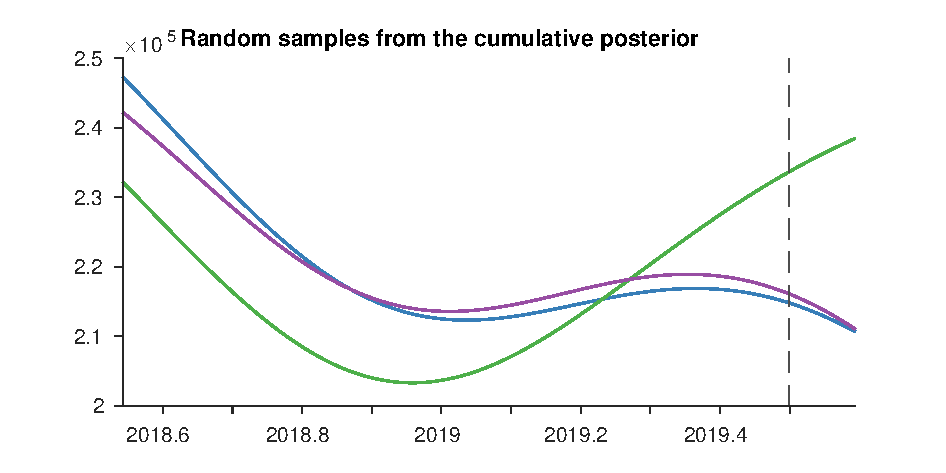
\includegraphics[width=\wmgd,height=\hmgd]{\mdrd/stocks-0-hyundaimobis_1_cum_sample}
\end{tabular}
\caption{Posterior of component 1 (top) and cumulative sum of components (bottom) with extrapolation. Mean and pointwise variance (left) and three random samples from the posterior distribution (right).}
\label{fig:extrap1}
\end{figure}

\subsection{Component 2 : A smooth function. This function applies from 20 Sep 2018 until 21 Nov 2018 and from 21 Nov 2018 until 29 Nov 2018}

This component is assumed to stop before the end of the data and will therefore be extrapolated as zero.

\begin{figure}[H]
\newcommand{\wmgd}{0.5\columnwidth}
\newcommand{\hmgd}{3.0cm}
\newcommand{\mdrd}{stocks-0-hyundaimobis}
\newcommand{\mbm}{\hspace{-0.3cm}}
\begin{tabular}{cc}
\mbm 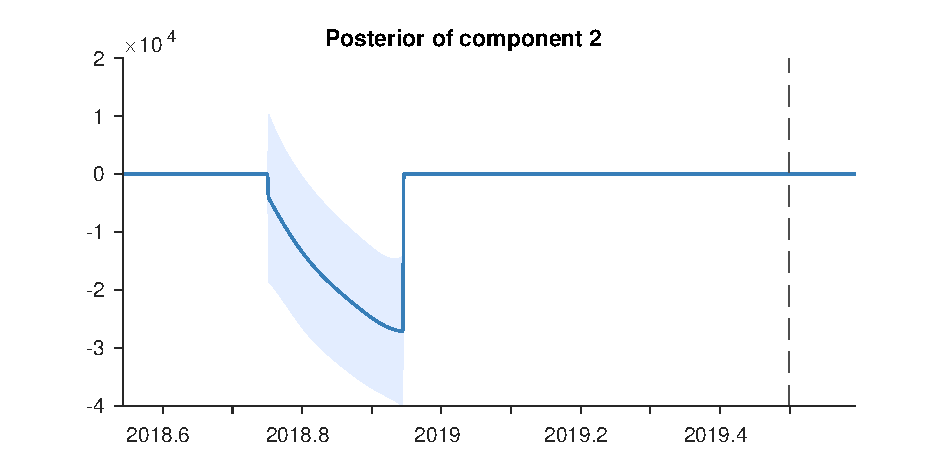
\includegraphics[width=\wmgd,height=\hmgd]{\mdrd/stocks-0-hyundaimobis_2_extrap} & 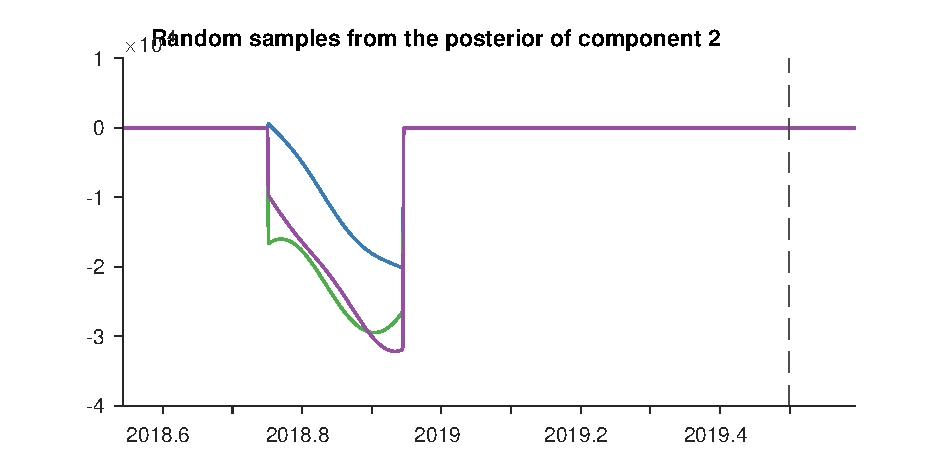
\includegraphics[width=\wmgd,height=\hmgd]{\mdrd/stocks-0-hyundaimobis_2_sample} \\
\mbm 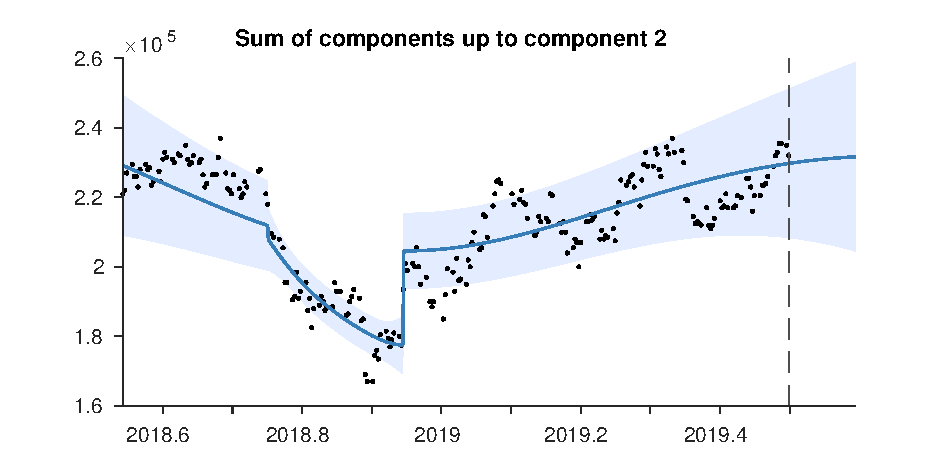
\includegraphics[width=\wmgd,height=\hmgd]{\mdrd/stocks-0-hyundaimobis_2_cum_extrap} & 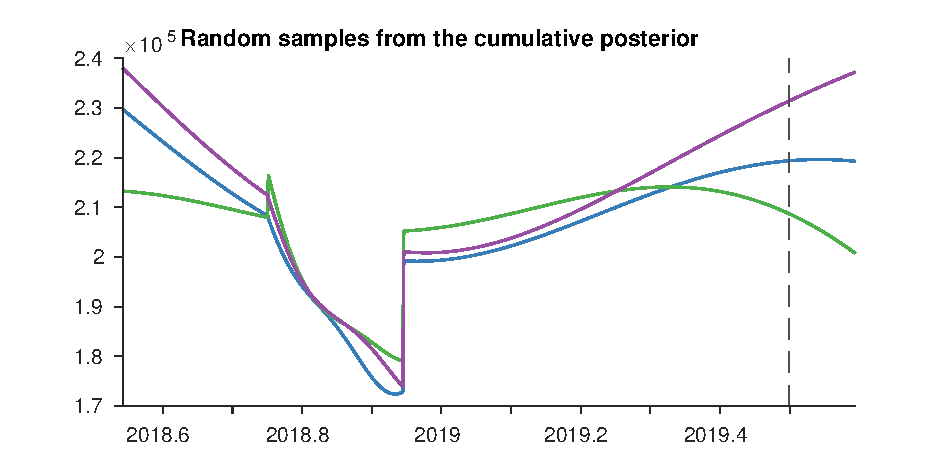
\includegraphics[width=\wmgd,height=\hmgd]{\mdrd/stocks-0-hyundaimobis_2_cum_sample}
\end{tabular}
\caption{Posterior of component 2 (top) and cumulative sum of components (bottom) with extrapolation. Mean and pointwise variance (left) and three random samples from the posterior distribution (right).}
\label{fig:extrap2}
\end{figure}

\subsection{Component 3 : A smooth function. This function applies until 20 Sep 2018 and from 29 Nov 2018 onwards}

This component is assumed to continue smoothly but is also assumed to be stationary so its distribution will return to the prior.
The prior distribution places mass on smooth functions with a marginal mean of zero and a typical lengthscale of 3.1 weeks.
[This is a placeholder for a description of how quickly the posterior will start to resemble the prior].

\begin{figure}[H]
\newcommand{\wmgd}{0.5\columnwidth}
\newcommand{\hmgd}{3.0cm}
\newcommand{\mdrd}{stocks-0-hyundaimobis}
\newcommand{\mbm}{\hspace{-0.3cm}}
\begin{tabular}{cc}
\mbm 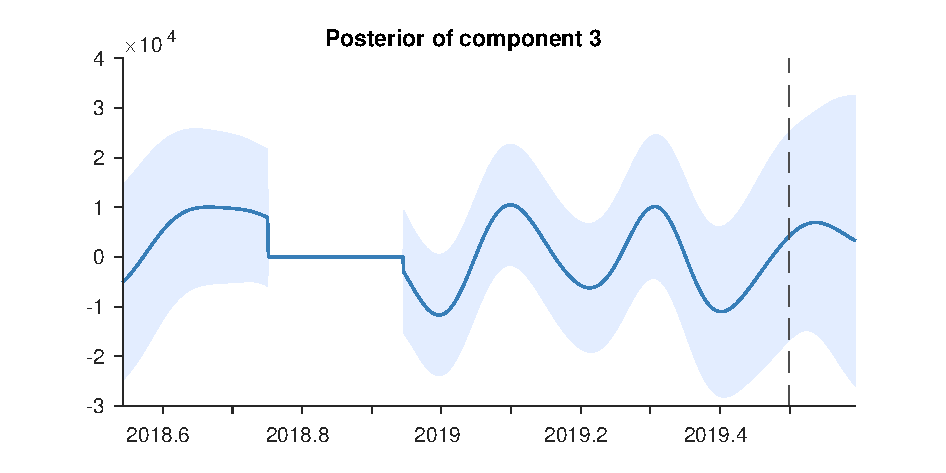
\includegraphics[width=\wmgd,height=\hmgd]{\mdrd/stocks-0-hyundaimobis_3_extrap} & 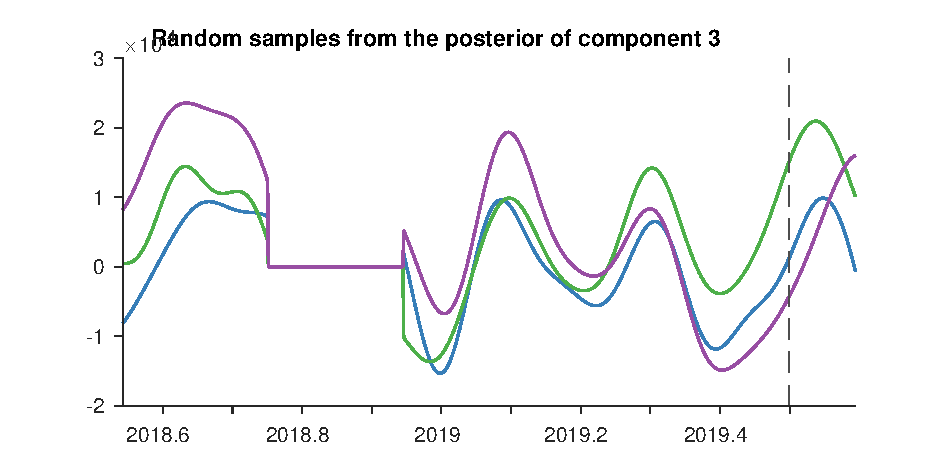
\includegraphics[width=\wmgd,height=\hmgd]{\mdrd/stocks-0-hyundaimobis_3_sample} \\
\mbm 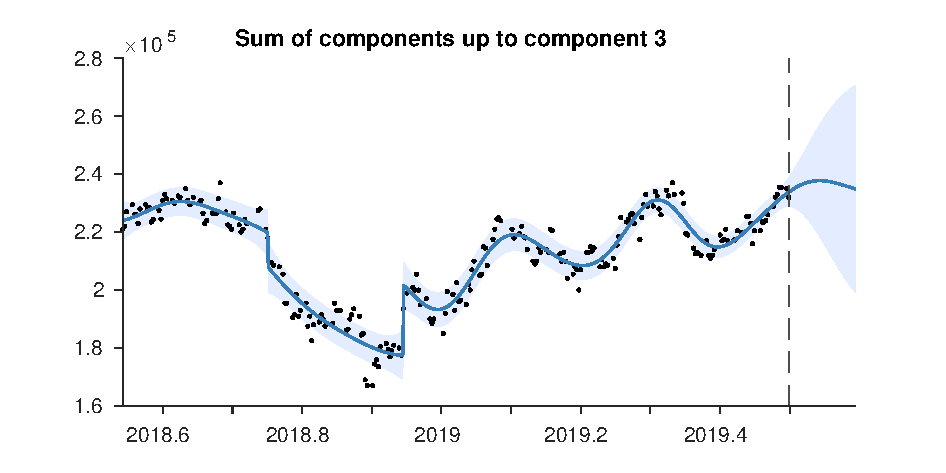
\includegraphics[width=\wmgd,height=\hmgd]{\mdrd/stocks-0-hyundaimobis_3_cum_extrap} & 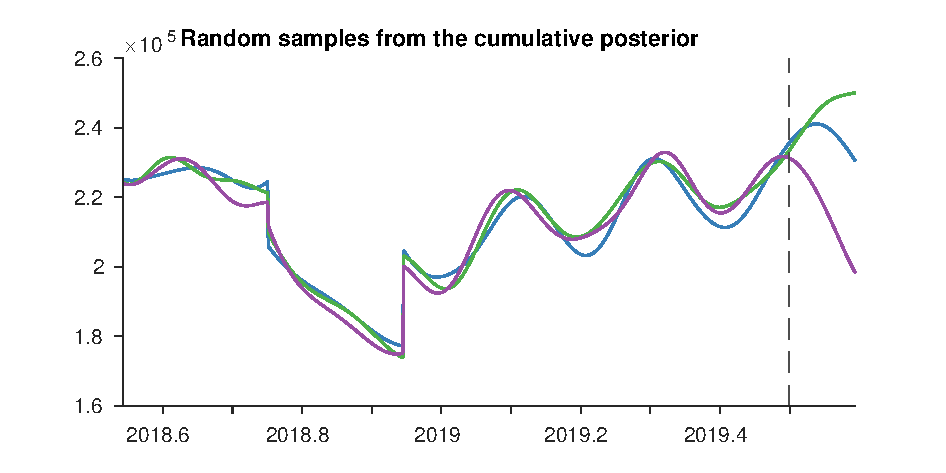
\includegraphics[width=\wmgd,height=\hmgd]{\mdrd/stocks-0-hyundaimobis_3_cum_sample}
\end{tabular}
\caption{Posterior of component 3 (top) and cumulative sum of components (bottom) with extrapolation. Mean and pointwise variance (left) and three random samples from the posterior distribution (right).}
\label{fig:extrap3}
\end{figure}

\subsection{Component 4 : A smooth function. This function applies from 21 Nov 2018 until 21 Nov 2018}

This component is assumed to stop before the end of the data and will therefore be extrapolated as zero.

\begin{figure}[H]
\newcommand{\wmgd}{0.5\columnwidth}
\newcommand{\hmgd}{3.0cm}
\newcommand{\mdrd}{stocks-0-hyundaimobis}
\newcommand{\mbm}{\hspace{-0.3cm}}
\begin{tabular}{cc}
\mbm 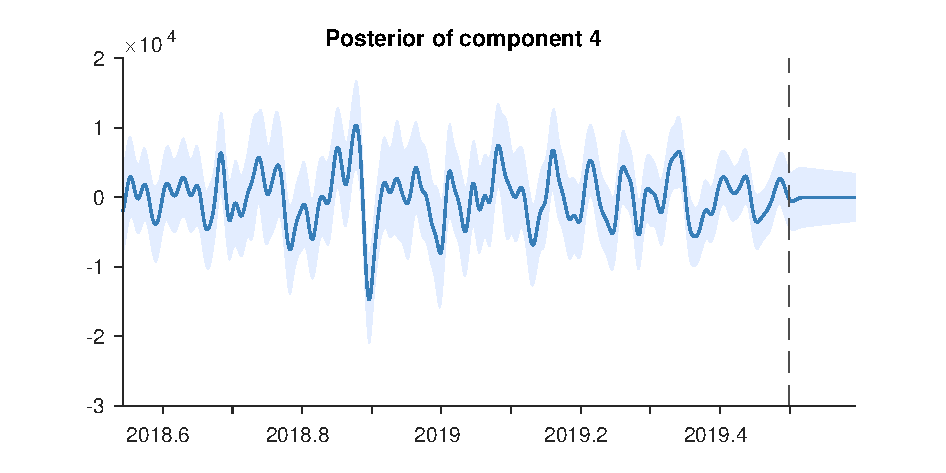
\includegraphics[width=\wmgd,height=\hmgd]{\mdrd/stocks-0-hyundaimobis_4_extrap} & 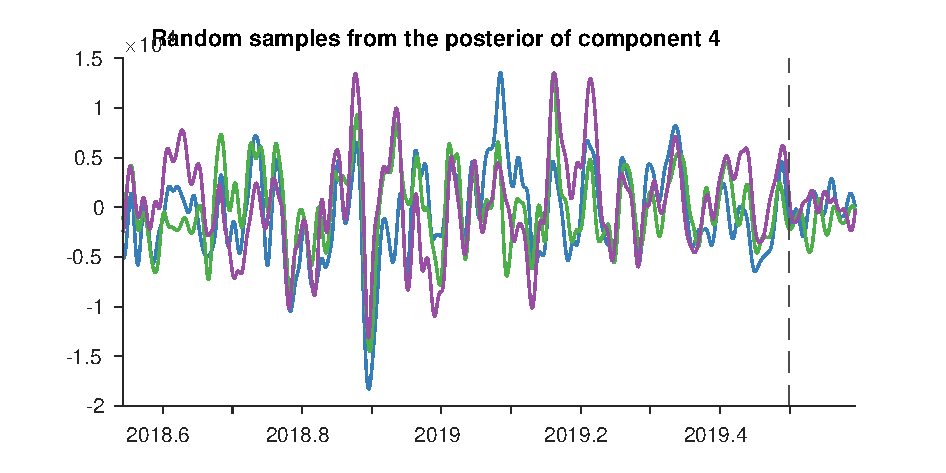
\includegraphics[width=\wmgd,height=\hmgd]{\mdrd/stocks-0-hyundaimobis_4_sample} \\
\mbm 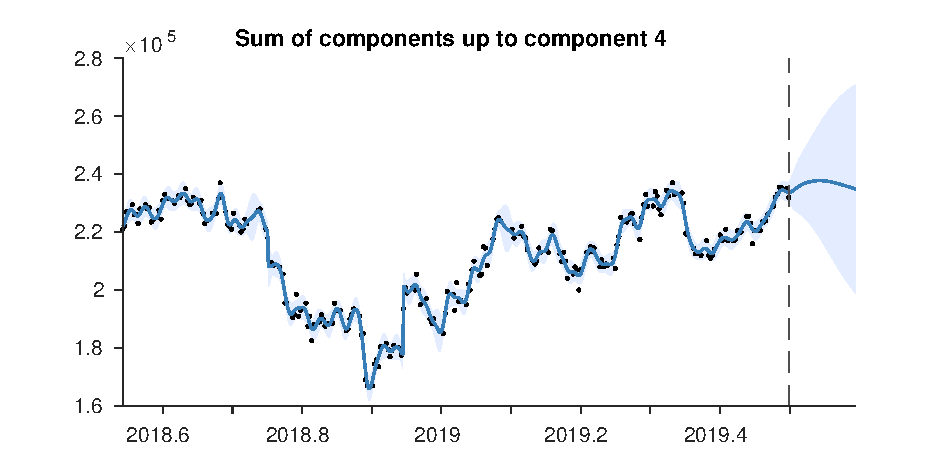
\includegraphics[width=\wmgd,height=\hmgd]{\mdrd/stocks-0-hyundaimobis_4_cum_extrap} & 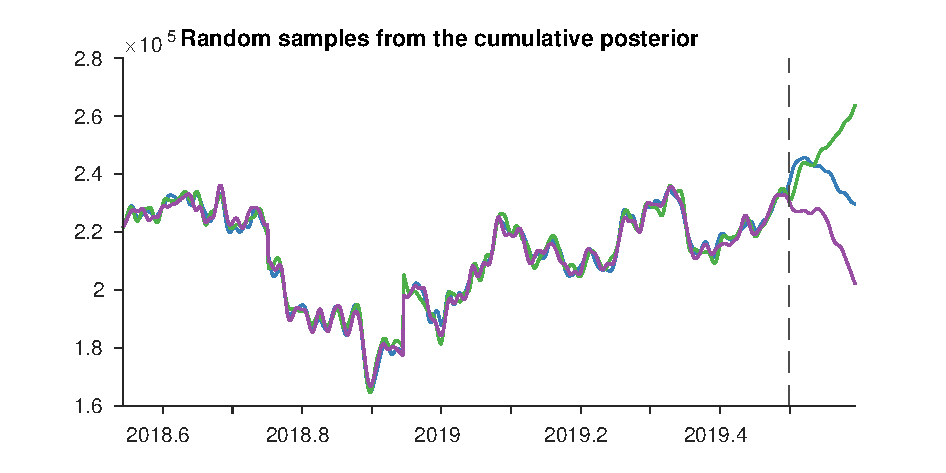
\includegraphics[width=\wmgd,height=\hmgd]{\mdrd/stocks-0-hyundaimobis_4_cum_sample}
\end{tabular}
\caption{Posterior of component 4 (top) and cumulative sum of components (bottom) with extrapolation. Mean and pointwise variance (left) and three random samples from the posterior distribution (right).}
\label{fig:extrap4}
\end{figure}

\subsection{Component 5 : Uncorrelated noise}

This component assumes the uncorrelated noise will continue indefinitely.

\begin{figure}[H]
\newcommand{\wmgd}{0.5\columnwidth}
\newcommand{\hmgd}{3.0cm}
\newcommand{\mdrd}{stocks-0-hyundaimobis}
\newcommand{\mbm}{\hspace{-0.3cm}}
\begin{tabular}{cc}
\mbm 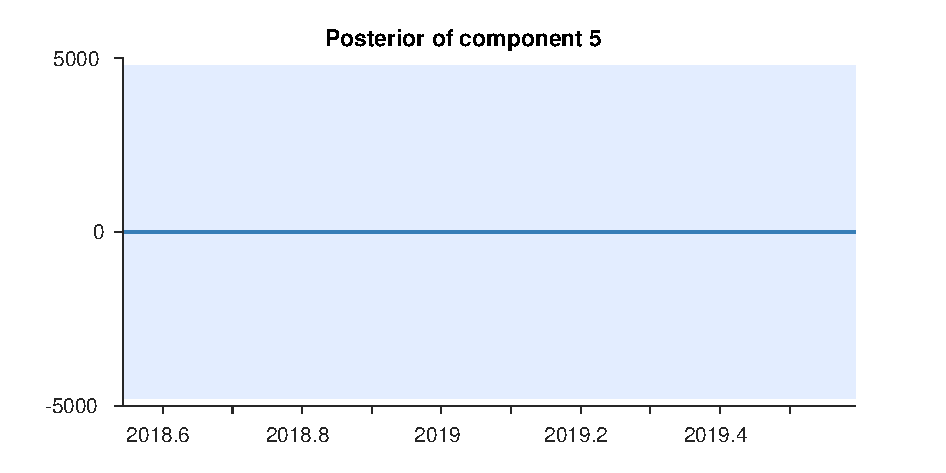
\includegraphics[width=\wmgd,height=\hmgd]{\mdrd/stocks-0-hyundaimobis_5_extrap} & 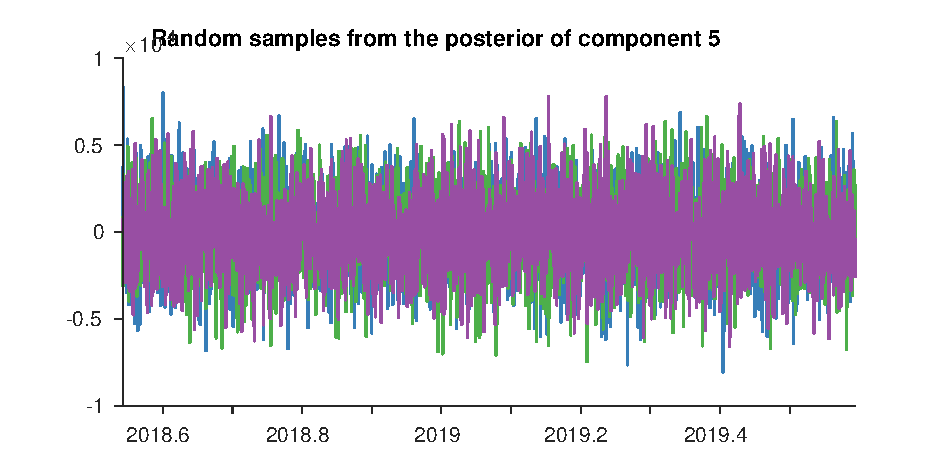
\includegraphics[width=\wmgd,height=\hmgd]{\mdrd/stocks-0-hyundaimobis_5_sample} \\
\mbm 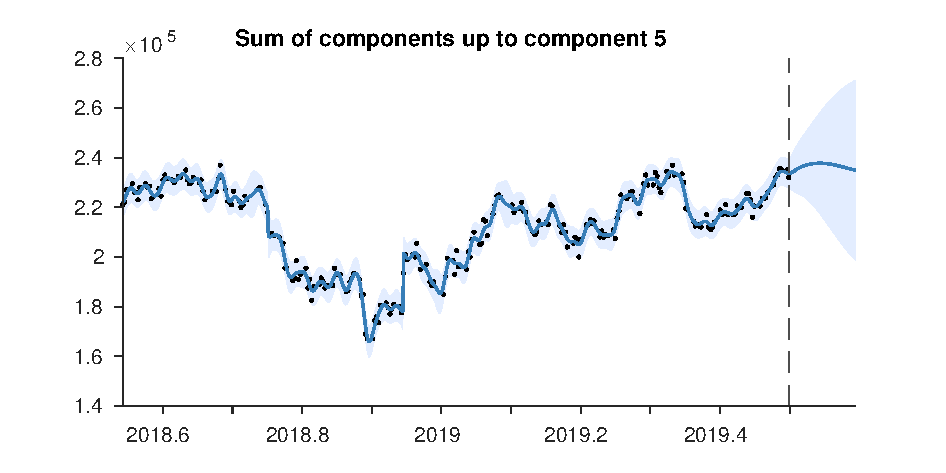
\includegraphics[width=\wmgd,height=\hmgd]{\mdrd/stocks-0-hyundaimobis_5_cum_extrap} & 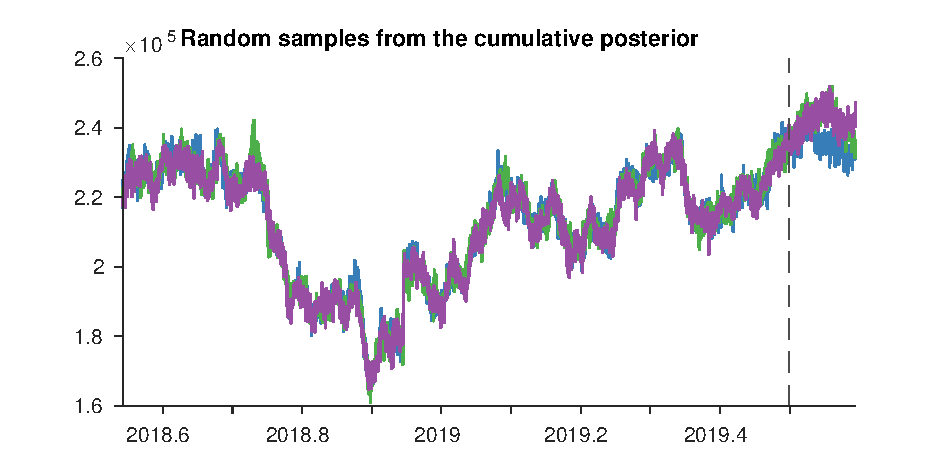
\includegraphics[width=\wmgd,height=\hmgd]{\mdrd/stocks-0-hyundaimobis_5_cum_sample}
\end{tabular}
\caption{Posterior of component 5 (top) and cumulative sum of components (bottom) with extrapolation. Mean and pointwise variance (left) and three random samples from the posterior distribution (right).}
\label{fig:extrap5}
\end{figure}

\subsection{Component 6 : A constant}

This component is assumed to stay constant.

\begin{figure}[H]
\newcommand{\wmgd}{0.5\columnwidth}
\newcommand{\hmgd}{3.0cm}
\newcommand{\mdrd}{stocks-0-hyundaimobis}
\newcommand{\mbm}{\hspace{-0.3cm}}
\begin{tabular}{cc}
\mbm 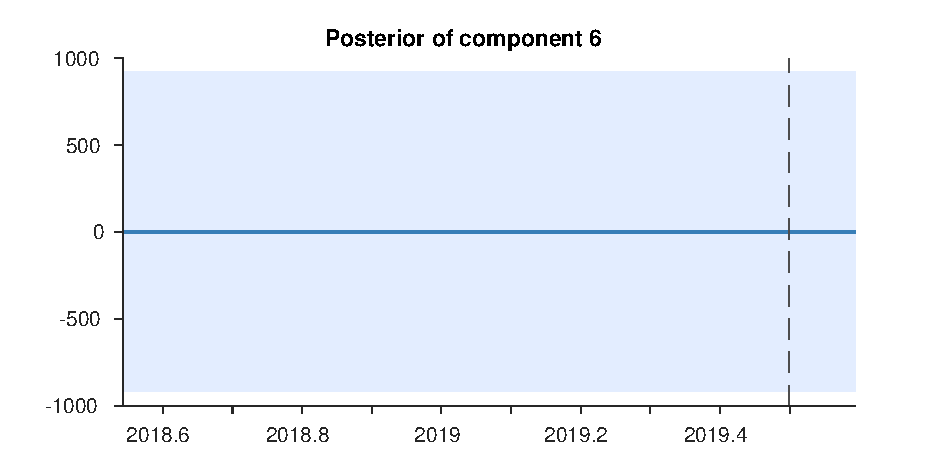
\includegraphics[width=\wmgd,height=\hmgd]{\mdrd/stocks-0-hyundaimobis_6_extrap} & 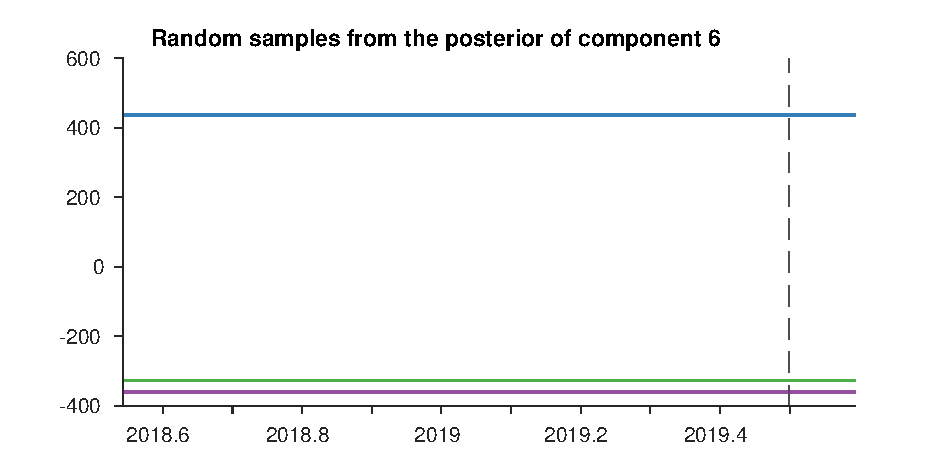
\includegraphics[width=\wmgd,height=\hmgd]{\mdrd/stocks-0-hyundaimobis_6_sample} \\
\mbm 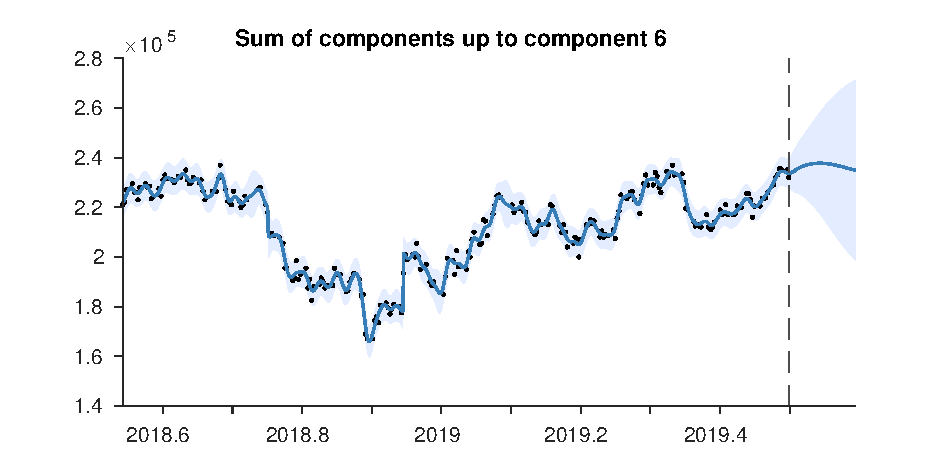
\includegraphics[width=\wmgd,height=\hmgd]{\mdrd/stocks-0-hyundaimobis_6_cum_extrap} & 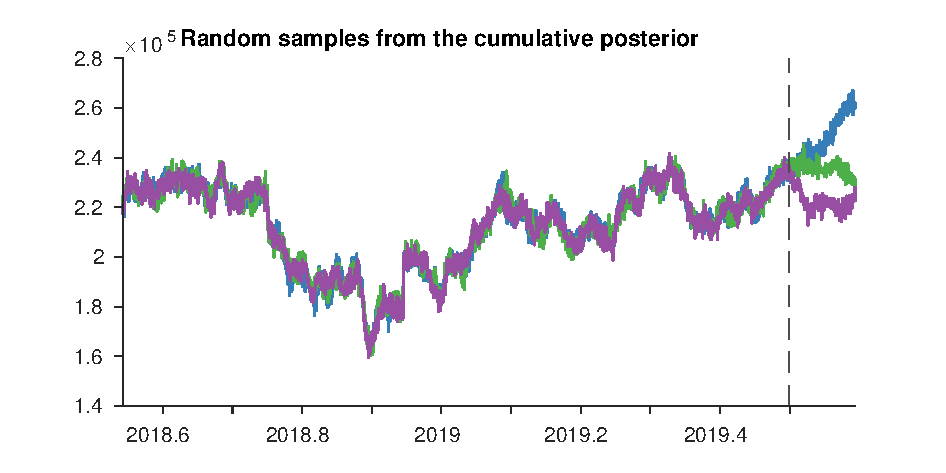
\includegraphics[width=\wmgd,height=\hmgd]{\mdrd/stocks-0-hyundaimobis_6_cum_sample}
\end{tabular}
\caption{Posterior of component 6 (top) and cumulative sum of components (bottom) with extrapolation. Mean and pointwise variance (left) and three random samples from the posterior distribution (right).}
\label{fig:extrap6}
\end{figure}

\section{Model checking}
\label{sec:check}

Several posterior predictive checks have been performed to assess how well the model describes the observed data.
These tests take the form of comparing statistics evaluated on samples from the prior and posterior distributions for each additive component.
The statistics are derived from autocorrelation function (ACF) estimates, periodograms and quantile-quantile (qq) plots.

Table~\ref{table:check} displays cumulative probability and $p$-value estimates for these quantities.
Cumulative probabilities near 0/1 indicate that the test statistic was lower/higher under the posterior compared to the prior unexpectedly often \ie they contain the same information as a $p$-value for a two-tailed test and they also express if the test statistic was higher or lower than expected.
$p$-values near 0 indicate that the test statistic was larger in magnitude under the posterior compared to the prior unexpectedly often.

\begin{table}[htb]
\begin{center}
{\small
\begin{tabular}{|r|rr|rr|rr|}
\hline
 & \multicolumn{2}{|c|}{ACF} & \multicolumn{2}{|c|}{Periodogram} & \multicolumn{2}{|c|}{QQ} \\
\bf{\#} & {min} & {min loc} & {max} & {max loc} & {max} & {min}\\
\hline

1 & \textcolor{gray}{0.167} & \textcolor{gray}{0.086} & \textcolor{gray}{0.786} & \textcolor{gray}{0.434} & \textcolor{gray}{0.081} & \textcolor{gray}{0.879}\\

2 & \textcolor{gray}{0.573} & \textcolor{gray}{0.722} & \textcolor{gray}{0.601} & \textcolor{gray}{0.347} & \textcolor{gray}{0.743} & \textcolor{gray}{0.148}\\

3 & \textcolor{gray}{0.398} & \textcolor{gray}{0.499} & \textcolor{gray}{0.266} & \textcolor{gray}{0.503} & \textcolor{gray}{0.303} & \textcolor{gray}{0.319}\\

4 & \textcolor{gray}{0.574} & \textcolor{gray}{0.607} & \textcolor{gray}{0.484} & \textcolor{gray}{0.421} & \textcolor{gray}{0.585} & \textcolor{gray}{0.486}\\

5 & \textcolor{gray}{0.506} & \textcolor{gray}{0.522} & \textcolor{gray}{0.488} & \textcolor{gray}{0.498} & \textcolor{gray}{0.523} & \textcolor{gray}{0.493}\\

6 & \textcolor{gray}{0.523} & \textcolor{gray}{0.512} & \textcolor{gray}{0.508} & \textcolor{gray}{0.492} & \textcolor{gray}{0.476} & \textcolor{gray}{0.524}\\

\hline
\end{tabular}
\caption{
Model checking statistics for each component.
Cumulative probabilities for minimum of autocorrelation function (ACF) and its location.
Cumulative probabilities for maximum of periodogram and its location.
$p$-values for maximum and minimum deviations of QQ-plot from straight line.
}
\label{table:check}
}
\end{center}
\end{table}

No statistically significant discrepancies between the data and model have been detected but model checking plots for each component are presented below.

\subsection{Model checking plots for components without statistically significant discrepancies}

\subsubsection{Component 1 : A very smooth function. This function applies until 21 Nov 2018 and from 21 Nov 2018 onwards}

No discrepancies between the prior and posterior of this component have been detected

\begin{figure}[H]
\newcommand{\wmgd}{0.5\columnwidth}
\newcommand{\hmgd}{3.0cm}
\newcommand{\mdrd}{stocks-0-hyundaimobis}
\newcommand{\mbm}{\hspace{-0.3cm}}
\begin{tabular}{cc}
\mbm 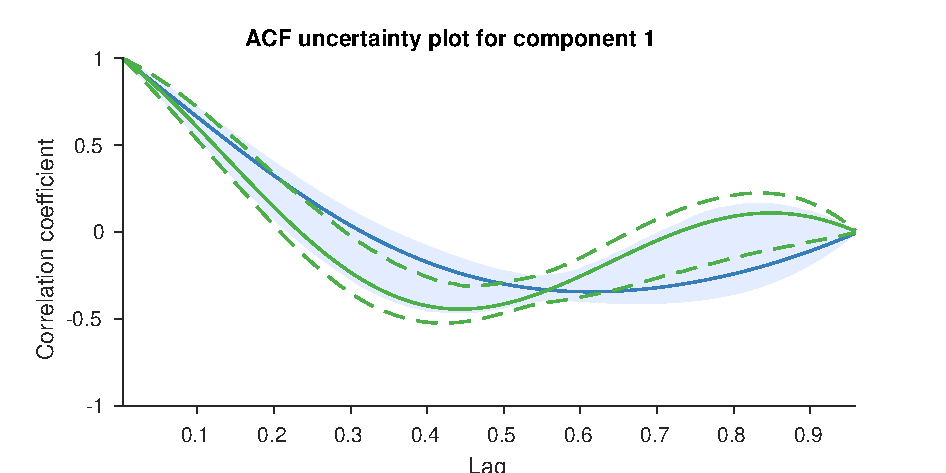
\includegraphics[width=\wmgd,height=\hmgd]{\mdrd/stocks-0-hyundaimobis_acf_bands_1} & 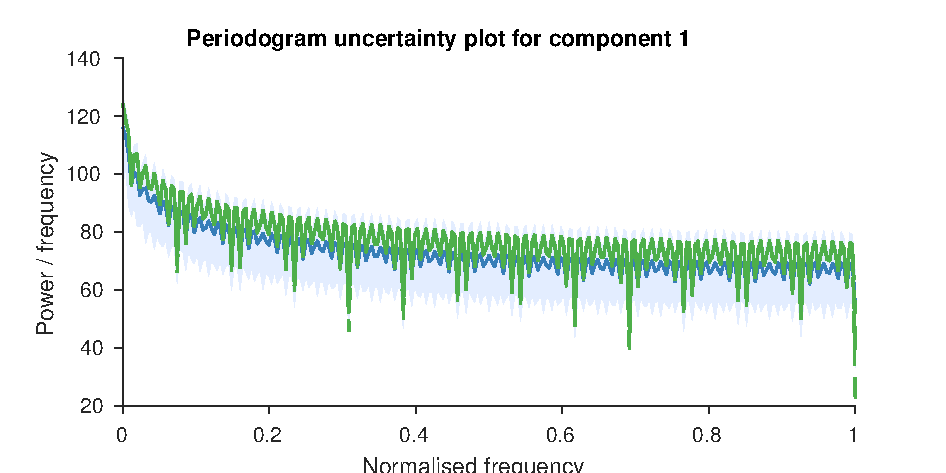
\includegraphics[width=\wmgd,height=\hmgd]{\mdrd/stocks-0-hyundaimobis_pxx_bands_1} \\
\mbm 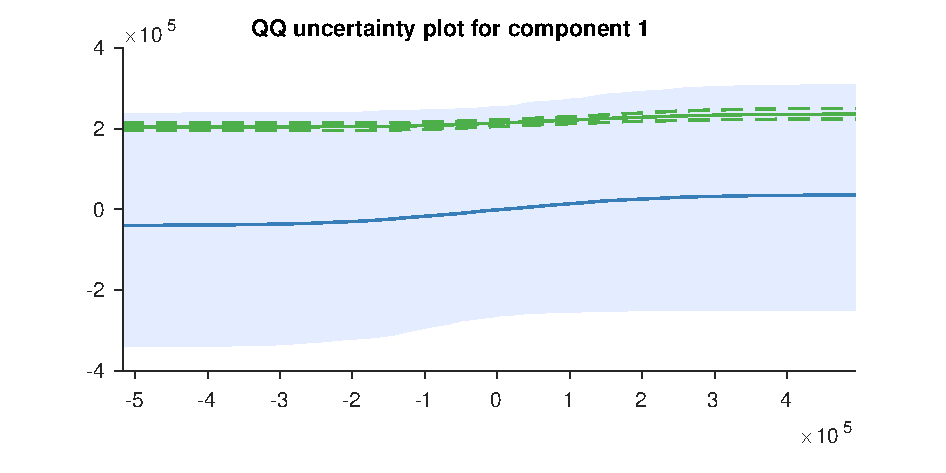
\includegraphics[width=\wmgd,height=\hmgd]{\mdrd/stocks-0-hyundaimobis_qq_bands_1}
\end{tabular}
\caption{
ACF (top left), periodogram (top right) and quantile-quantile (bottom left) uncertainty plots.
The blue line and shading are the pointwise mean and 90\% confidence interval of the plots under the prior distribution for component 1.
The green line and green dashed lines are the corresponding quantities under the posterior.}
\label{fig:check1}
\end{figure}

\subsubsection{Component 2 : A smooth function. This function applies from 20 Sep 2018 until 21 Nov 2018 and from 21 Nov 2018 until 29 Nov 2018}

No discrepancies between the prior and posterior of this component have been detected

\begin{figure}[H]
\newcommand{\wmgd}{0.5\columnwidth}
\newcommand{\hmgd}{3.0cm}
\newcommand{\mdrd}{stocks-0-hyundaimobis}
\newcommand{\mbm}{\hspace{-0.3cm}}
\begin{tabular}{cc}
\mbm 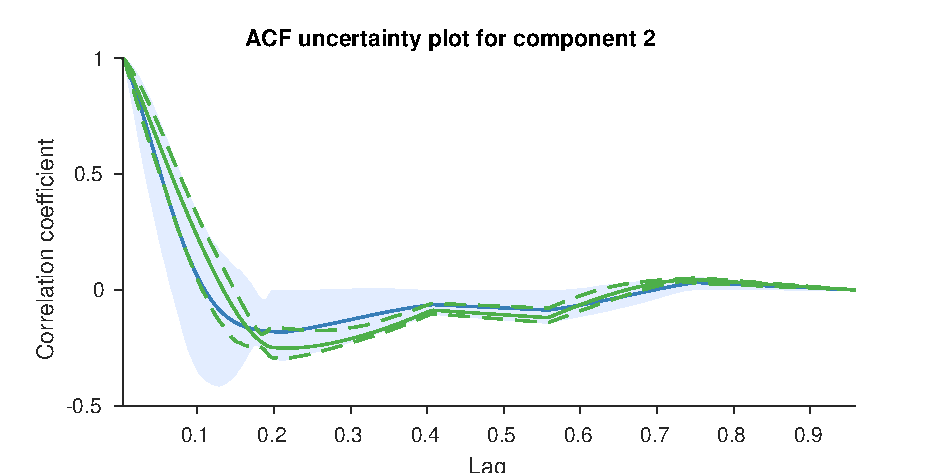
\includegraphics[width=\wmgd,height=\hmgd]{\mdrd/stocks-0-hyundaimobis_acf_bands_2} & 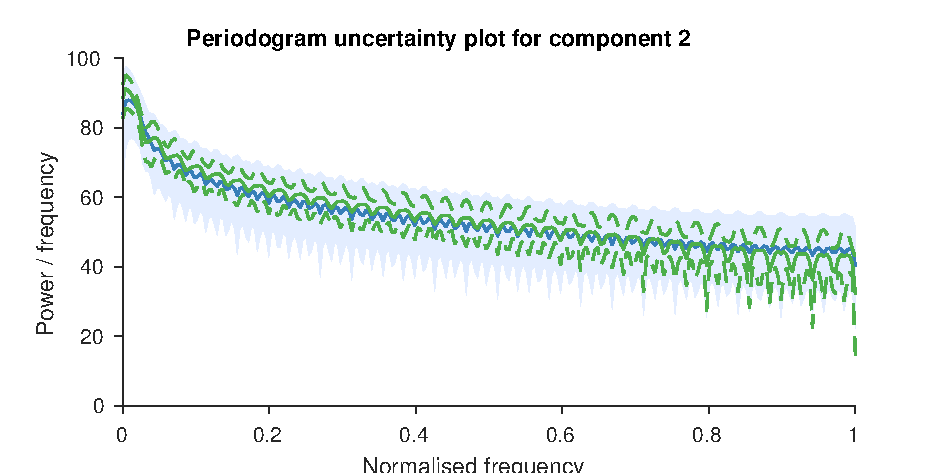
\includegraphics[width=\wmgd,height=\hmgd]{\mdrd/stocks-0-hyundaimobis_pxx_bands_2} \\
\mbm \includegraphics[width=\wmgd,height=\hmgd]{\mdrd/stocks-0-hyundaimobis_qq_bands_2}
\end{tabular}
\caption{
ACF (top left), periodogram (top right) and quantile-quantile (bottom left) uncertainty plots.
The blue line and shading are the pointwise mean and 90\% confidence interval of the plots under the prior distribution for component 2.
The green line and green dashed lines are the corresponding quantities under the posterior.}
\label{fig:check2}
\end{figure}

\subsubsection{Component 3 : A smooth function. This function applies until 20 Sep 2018 and from 29 Nov 2018 onwards}

No discrepancies between the prior and posterior of this component have been detected

\begin{figure}[H]
\newcommand{\wmgd}{0.5\columnwidth}
\newcommand{\hmgd}{3.0cm}
\newcommand{\mdrd}{stocks-0-hyundaimobis}
\newcommand{\mbm}{\hspace{-0.3cm}}
\begin{tabular}{cc}
\mbm \includegraphics[width=\wmgd,height=\hmgd]{\mdrd/stocks-0-hyundaimobis_acf_bands_3} & \includegraphics[width=\wmgd,height=\hmgd]{\mdrd/stocks-0-hyundaimobis_pxx_bands_3} \\
\mbm \includegraphics[width=\wmgd,height=\hmgd]{\mdrd/stocks-0-hyundaimobis_qq_bands_3}
\end{tabular}
\caption{
ACF (top left), periodogram (top right) and quantile-quantile (bottom left) uncertainty plots.
The blue line and shading are the pointwise mean and 90\% confidence interval of the plots under the prior distribution for component 3.
The green line and green dashed lines are the corresponding quantities under the posterior.}
\label{fig:check3}
\end{figure}

\subsubsection{Component 4 : A smooth function. This function applies from 21 Nov 2018 until 21 Nov 2018}

No discrepancies between the prior and posterior of this component have been detected

\begin{figure}[H]
\newcommand{\wmgd}{0.5\columnwidth}
\newcommand{\hmgd}{3.0cm}
\newcommand{\mdrd}{stocks-0-hyundaimobis}
\newcommand{\mbm}{\hspace{-0.3cm}}
\begin{tabular}{cc}
\mbm \includegraphics[width=\wmgd,height=\hmgd]{\mdrd/stocks-0-hyundaimobis_acf_bands_4} & \includegraphics[width=\wmgd,height=\hmgd]{\mdrd/stocks-0-hyundaimobis_pxx_bands_4} \\
\mbm \includegraphics[width=\wmgd,height=\hmgd]{\mdrd/stocks-0-hyundaimobis_qq_bands_4}
\end{tabular}
\caption{
ACF (top left), periodogram (top right) and quantile-quantile (bottom left) uncertainty plots.
The blue line and shading are the pointwise mean and 90\% confidence interval of the plots under the prior distribution for component 4.
The green line and green dashed lines are the corresponding quantities under the posterior.}
\label{fig:check4}
\end{figure}

\subsubsection{Component 5 : Uncorrelated noise}

No discrepancies between the prior and posterior of this component have been detected

\begin{figure}[H]
\newcommand{\wmgd}{0.5\columnwidth}
\newcommand{\hmgd}{3.0cm}
\newcommand{\mdrd}{stocks-0-hyundaimobis}
\newcommand{\mbm}{\hspace{-0.3cm}}
\begin{tabular}{cc}
\mbm \includegraphics[width=\wmgd,height=\hmgd]{\mdrd/stocks-0-hyundaimobis_acf_bands_5} & \includegraphics[width=\wmgd,height=\hmgd]{\mdrd/stocks-0-hyundaimobis_pxx_bands_5} \\
\mbm \includegraphics[width=\wmgd,height=\hmgd]{\mdrd/stocks-0-hyundaimobis_qq_bands_5}
\end{tabular}
\caption{
ACF (top left), periodogram (top right) and quantile-quantile (bottom left) uncertainty plots.
The blue line and shading are the pointwise mean and 90\% confidence interval of the plots under the prior distribution for component 5.
The green line and green dashed lines are the corresponding quantities under the posterior.}
\label{fig:check5}
\end{figure}

\subsubsection{Component 6 : A constant}

No discrepancies between the prior and posterior of this component have been detected

\begin{figure}[H]
\newcommand{\wmgd}{0.5\columnwidth}
\newcommand{\hmgd}{3.0cm}
\newcommand{\mdrd}{stocks-0-hyundaimobis}
\newcommand{\mbm}{\hspace{-0.3cm}}
\begin{tabular}{cc}
\mbm \includegraphics[width=\wmgd,height=\hmgd]{\mdrd/stocks-0-hyundaimobis_acf_bands_6} & \includegraphics[width=\wmgd,height=\hmgd]{\mdrd/stocks-0-hyundaimobis_pxx_bands_6} \\
\mbm \includegraphics[width=\wmgd,height=\hmgd]{\mdrd/stocks-0-hyundaimobis_qq_bands_6}
\end{tabular}
\caption{
ACF (top left), periodogram (top right) and quantile-quantile (bottom left) uncertainty plots.
The blue line and shading are the pointwise mean and 90\% confidence interval of the plots under the prior distribution for component 6.
The green line and green dashed lines are the corresponding quantities under the posterior.}
\label{fig:check6}
\end{figure}

\section{MMD - experimental section}
\label{sec:mmd}

\begin{table}[htb]
\begin{center}
{\small
\begin{tabular}{|r|r|}
\hline
\bf{\#} & {mmd}\\
\hline

1 & \textbf{0.000}\\

2 & \textbf{0.002}\\

3 & \textbf{0.000}\\

4 & \textbf{0.000}\\

5 & 0.046\\

6 & \textcolor{gray}{0.090}\\

\hline
\end{tabular}
\caption{
MMD $p$-values
}
\label{table:mmd}
}
\end{center}
\end{table}

\subsubsection{Component 1 : A very smooth function. This function applies until 21 Nov 2018 and from 21 Nov 2018 onwards}

\begin{figure}[H]
\newcommand{\wmgd}{0.5\columnwidth}
\newcommand{\hmgd}{3.0cm}
\newcommand{\mdrd}{stocks-0-hyundaimobis}
\newcommand{\mbm}{\hspace{-0.3cm}}
\includegraphics[width=\wmgd,height=\hmgd]{\mdrd/stocks-0-hyundaimobis_mmd_1}
\caption{
MMD plot}
\label{fig:mmd1}
\end{figure}

\subsubsection{Component 2 : A smooth function. This function applies from 20 Sep 2018 until 21 Nov 2018 and from 21 Nov 2018 until 29 Nov 2018}

\begin{figure}[H]
\newcommand{\wmgd}{0.5\columnwidth}
\newcommand{\hmgd}{3.0cm}
\newcommand{\mdrd}{stocks-0-hyundaimobis}
\newcommand{\mbm}{\hspace{-0.3cm}}
\includegraphics[width=\wmgd,height=\hmgd]{\mdrd/stocks-0-hyundaimobis_mmd_2}
\caption{
MMD plot}
\label{fig:mmd2}
\end{figure}

\subsubsection{Component 3 : A smooth function. This function applies until 20 Sep 2018 and from 29 Nov 2018 onwards}

\begin{figure}[H]
\newcommand{\wmgd}{0.5\columnwidth}
\newcommand{\hmgd}{3.0cm}
\newcommand{\mdrd}{stocks-0-hyundaimobis}
\newcommand{\mbm}{\hspace{-0.3cm}}
\includegraphics[width=\wmgd,height=\hmgd]{\mdrd/stocks-0-hyundaimobis_mmd_3}
\caption{
MMD plot}
\label{fig:mmd3}
\end{figure}

\subsubsection{Component 4 : A smooth function. This function applies from 21 Nov 2018 until 21 Nov 2018}

\begin{figure}[H]
\newcommand{\wmgd}{0.5\columnwidth}
\newcommand{\hmgd}{3.0cm}
\newcommand{\mdrd}{stocks-0-hyundaimobis}
\newcommand{\mbm}{\hspace{-0.3cm}}
\includegraphics[width=\wmgd,height=\hmgd]{\mdrd/stocks-0-hyundaimobis_mmd_4}
\caption{
MMD plot}
\label{fig:mmd4}
\end{figure}

\subsubsection{Component 5 : Uncorrelated noise}

\begin{figure}[H]
\newcommand{\wmgd}{0.5\columnwidth}
\newcommand{\hmgd}{3.0cm}
\newcommand{\mdrd}{stocks-0-hyundaimobis}
\newcommand{\mbm}{\hspace{-0.3cm}}
\includegraphics[width=\wmgd,height=\hmgd]{\mdrd/stocks-0-hyundaimobis_mmd_5}
\caption{
MMD plot}
\label{fig:mmd5}
\end{figure}

\subsubsection{Component 6 : A constant}

\begin{figure}[H]
\newcommand{\wmgd}{0.5\columnwidth}
\newcommand{\hmgd}{3.0cm}
\newcommand{\mdrd}{stocks-0-hyundaimobis}
\newcommand{\mbm}{\hspace{-0.3cm}}
\includegraphics[width=\wmgd,height=\hmgd]{\mdrd/stocks-0-hyundaimobis_mmd_6}
\caption{
MMD plot}
\label{fig:mmd6}
\end{figure}

\end{document}
